%!TEX root = ../thesis.tex  % Comment this line for standalone compilation
%*******************************************************************************
%*********************************** First Chapter *****************************
%*******************************************************************************

\chapter{CAFLOW: Conditional Autoregressive Flows} \label{Chapter:CAFLOW}  %Title of the First Chapter

\ifpdf
    \graphicspath{{Chapter1/Figs/Raster/}{Chapter1/Figs/PDF/}{Chapter1/Figs/}}
\else
    \graphicspath{{Chapter1/Figs/Vector/}{Chapter1/Figs/}}
\fi

In this chapter, we introduce CAFLOW, a new diverse image-to-image translation model that simultaneously leverages the power of autoregressive modeling and the modeling efficiency of conditional normalizing flows. We transform the conditioning image into a sequence of latent encodings using a multi-scale normalizing flow and repeat the process for the conditioned image. We model the conditional distribution of the latent encodings by modeling the autoregressive distributions with an efficient multi-scale normalizing flow, where each conditioning factor affects image synthesis at its respective resolution scale. Our proposed framework performs well on a range of image-to-image translation tasks. It outperforms former designs of conditional flows because of its expressive autoregressive structure.

%********************************** %First Section  **************************************
\section{Introduction}

Generative modeling has emerged as one of the most widely-researched areas in deep learning over the last few years. While generative adversarial networks (GANs) \cite{GANs} produce state-of-the-art results for images \cite{viazovetskyi2020stylegan2}, they do not allow for the estimation of likelihoods. Other types of generative methods, however, admit the explicit evaluation of likelihoods of points under the given model, and thus allow for training as maximum likelihood estimators. Normalizing flows \cite{rezende2015variational} (and their continuous formulation, via NeuralODEs \cite{neuralODEs}) are one such example. These \emph{flow-based} models are diffeomorphic neural networks, which are trained to invertibly transform data into e.g. a normal distribution. This is made possible by a change-of-variables formula, which expresses the likelihood of a data sample in terms of the normal distribution. Samples from the approximated distribution are then generated by passing samples from a normal distribution through the inverse function.

A straightforward extension of likelihood estimators are \emph{conditional} likelihood estimators, which represent the likelihood of a random variable conditioned on another random variable. This is in particular used in autoregressive models and their flow-based variants (\emph{autoregressive flows} \cite{autoregressive_flows}). These types of models explicitly parametrize joint likelihoods via the product rule for probability densities, and can hence be used for creating expressive likelihood estimators, at the cost of more involved computations. This approach is in particular employed by Wavelet Flows \cite{WAVELET-FLOW}, which use a hierarchical multi-scale representation via Wavelet decompositions in order to parametrize expressive conditional likelihood functions for images.

Conditional likelihood estimators are also used for domain transfer and image-to-image translation \cite{Dual-Glow, SRFLOW, ardizzone2019guided, cGLOW} achieving comparable performances to GAN-based models in super-resolution \cite{SRFLOW, HCFLOW}, inpainting \cite{cGLOW} and image-to-image translation \cite{Pumarola2020, Dual-Glow, grover2020alignflow}. In domain transfer, the task is to \emph{transfer} a data point from some \emph{origin} domain (e.g. black-and-white images) to a different \emph{target} domain, e.g. color images in this example. The technique of conditioning lends itself well to domain transfer, as it is possible to condition likelihood functions over the target domain on points from the origin domain, thereby making conditional generation possible. In flow-based models, this has been introduced in the form of conditional flows, which function based on this general principle. The most successful examples of conditional flows are \cite{SRFLOW} and \cite{HCFLOW} which achieved state-of-the-art performance in image super-resolution by adapting conditional flows to the task of image super-resolution. Both methods rely on powerful feature extractors specifically optimised for image super-resolution to extract conditional features from the low resolution image. This makes them not easily applicable to general inverse problem solving.

\medskip

\textbf{Outline of the main contributions}. In this chapter, we introduce CAFLOW, \emph{conditional autoregressive flow}, which combines the idea of conditional flows with the expressiveness of autoregressive models using hierarchical multi-scale flows for domain transfer. Our goal is to improve the performance of conditional flows on %general inverse problem solving 
general inverse problems in vision.\color{black}

As a first step, we encode the condition and the target images using invertible netchapters into a hierarchical sequence of $n$ latent spaces. Then, using the chain rule of probability, we decompose the conditional distribution of the latent encodings into $n$ autoregressive component distributions with the aim of modeling each distribution using a conditional normalizing flow. Modeling the theoretical autoregressive components can be computationally very expensive. For this reason, we used a small set of assumptions that allowed us to design a computationally efficient multiscale normalizing flow at a small modeling flexibility cost. By carefully designing such a flow based on weak assumptions on the mutual dependencies of the latent encodings, our model allows for exchange of information between latent spaces of different dimension. In particular, our designed architecture is able to capture correlations between different scales, improving on the expressivity of other conditional flow-based models used for domain transfer tasks. The training of the $n$ conditional flows can be parallelized, however, the sampling process is sequential and could become computationally expensive if the number of scales is large. However, in practice, the choice of the invertible netchapters that map the images to latent encodings does not allow the number of scales $n$ to be large, which makes the sampling time of CAFLOW much smaller than that of pure autoregressive models and slightly greater than that of standard conditional flows.

Our modeling choices are corroborated by strong experimental evidence. Using an ablation study, we confirmed experimentally that the autoregressive model outperforms the non-autoregressive model. Furthermore, we demonstrate that our model outperforms standard designs of conditional flows on classical image-to-image translation tasks such as image super-resolution, image colorization and image inpainting. In particular, we show that on these tasks CAFLOW outperforms former designs of conditional flows and GAN-based models thanks to its expressive autoregressive structure.

Concurrently to our chapter, Liang et al. \cite{HCFLOW} introduced autoregressive conditioning in the latent space, which yielded improved results compared to their earlier chapter \cite{SRFLOW}. 
However, they make the following restrictive modelling assumption: the low resolution image is part of the target latent space.  This makes their method not applicable to general inverse problems in vision. 

As far as inverse problems on other modalities are considered, our method can be suitably modified to address inverse problems on structured data where there is an underlying hierarchical decomposition of the signal. It is true that our method would not be easily applied in unstructured data such as categorical or tabular data. However, the same applies to all other conditional normalizing flow methods that use a multiscale structure.
\color{black}

\medskip

\textbf{Organization of the chapter.} The chapter is organized as follows.
In Section \ref{ch1:sec:background}, we provide the necessary theoretical background on unconditional and conditional normalizing flows. In Section \ref{ch1:sec:Caflow}, we describe our CAFLOW method discussing the modeling assumptions and deriving a formula for estimating the log-likelihood of the unknown conditional probability. In Section \ref{ch1:sec:numerics}, we present the quantitative and qualitative results of our experiments. Finally, in Sections \ref{ch1:sec:conclusions} we discuss the limitations of our chapter and we draw our conclusions. 

\section{Background}\label{ch1:sec:background}

\subsection{Notations}

Random variables will be denoted by capital letters, e.g. $X$, $Y$, while their associated probability will be indicated by $P(X)$, $P(Y)$ and their distributions by $p_X$ and $p_Y$. 
We use calligraphic capital letters, e.g. $\mathcal{X}, \mathcal{Y}$, to denote the sample space of the random variables $X$, $Y$ and small bold letters $\x$, $\y$ for the samples. Finally, given two random variables $X$ and $Y$ we will consider the conditional probability of $Y$ given $X$ and we denote it by $P(Y|X)$. Its density will be indicated by $p_{Y|X}$. We remark that throughout the chapter we will always implicitly assume that the considered probabilities admit a density.

\subsection{Normalizing flows}\label{ch1:subsec:normalizing}

Given a random variable $Y$ defined on $\mathcal{Y}$ with an unknown distribution $p_Y$, the main idea of flow-based generative modeling is to approximate $p_Y$ with a learned function $p^\theta_Y$, which is parametrized by an invertible neural netchapter $G^\theta$ mapping from a latent space $\mathcal{Z}$ to $\mathcal{Y}$. 
Choosing $P(Z)$ to be a probability associated to the random variable $Z$ and $p_Z$ its distribution on $\mathcal{Z}$, we define the function $p^\theta_Y$ as the distribution of the push-forward measure of $P_Z$ by the map $G^\theta$.
By the change-of-variables formula for probability distributions, $p^\theta_Y$ is easily computed as
\begin{align*}
p^\theta_Y(\y) = p_Z(F^\theta(\y)) \left| \det \left(\frac{d F^\theta(\y)}{d\y} \right)\right|,
\end{align*}
where $F^\theta$ is the inverse of $G^\theta$.
Thanks to the formula above it is then possible to match $p^\theta_Y$ to $p_Y$ by miminizing the negative log-likelihood of $p^\theta_Y$, defined as
\begin{align*}
- \log p^\theta_Y(\y) = -  \log(p_Z(F^\theta(\y))) -  \log\left| \det \left(\frac{d F^\theta(\y)}{d\y} \right)\right|.
\end{align*}
In practice, the transformation $G^\theta$ is a composition of learnable invertible transformations $G_{1}, ..., G_{n}$ such that $G_i : \mathcal{Z}_{i} \rightarrow \mathcal{Z}_{i+1}$ (where $\mathcal{Z}_1 = \mathcal{Z}$ and $\mathcal{Z}_{n+1} = \mathcal{Y}$) for intermediate latent spaces $\mathcal{Z}_i$ and
\begin{equation}
    \y = G_{n}(G_{n-1}(...G_{1}(\z)))=G^{\theta}(\z)\,, \quad  \z= F_1(F_{2}(...F_n(\y)))=F^{\theta}(\y),
\end{equation}
where $F_i = (G_i)^{-1}$ for every $i$ and thus $F^\theta = (G^\theta)^{-1}$ (Note that we are assuming implicitly that each $G_i$ and $F_i$ depends on $\theta$, but we drop the superscript $\theta$ for notational convenience). This model is called a normalizing flow.
In this case, using the properties of the Jacobian for composition of invertible transformations the log-likelihood of $p^\theta_Y$ can be computed as 
\begin{equation}\label{ch1:ch1:eq:loglike}
\log(p^\theta_Y(\y) ) = \log(p_Z(F^\theta(\y))) + \sum_{i=1}^{n}  \log\left| \det \left(\frac{d{F_i}(\z_{i+1})}{d\z_{i+1}} \right)\right|,
\end{equation}
where $\z_{n+1} = \y$.


In order to estimate $\log(p^\theta_Y(\y) )$ the transformations $G_i$ need to be designed to have a computable inverse $F_i$ and a tractable Jacobian determinant. 
%We next describe typical choices for the transformations $g_i$ introduced in \cite{Nice2014, GLOW} and then commonly used in most of the normalizing flow architectures. We will refer to them in the next sections where we describe our method.
We next present typical choices for the transformations $G_i$. We describe each method by presenting the forward transform $G_i$, the inverse transform $F_i$ and the  log-determinant of the Jacobian. The calculation of the Jacobian determinant is used in the calculation of the log-likelihood in \eqref{ch1:ch1:eq:loglike}.
\color{black}

\medskip

\textbf{Affine coupling layer}. Affine coupling layers \cite{Nice2014} capture complex dependencies of the activations in an invertible and computationally efficient way.

\smallskip

\textit{\underline{Forward Function}}:

A given a tensor \(\z\) is partitioned into two parts: \(\z_1\) and \(\z_2\). The tensor \(\z_2\) remains unchanged and is used in the transformation of \(\z_1\). A nonlinear mapping, represented by NN (typically a shallow convolutional neural netchapter), processes \(\z_2\) producing two outputs of the same dimension as \(\z_1\): \(\boldsymbol{u}\) and \(\boldsymbol{t}\). The exponential of \(\boldsymbol{u}\) is used as the scale and $\boldsymbol{t}$ as the bias of the affine transformation of \(\z_1\). The steps are the following:
\begin{align*}
\z_1, \z_2 &= \text{split}(\z) \\
(\boldsymbol{u},\boldsymbol{t}) &= NN(\z_2) \\
\s &= \exp(\boldsymbol{u}) \\
\y_1 &= \s \odot \z_1 + \boldsymbol{t} \\
\y_2 &= \z_2.
\end{align*}
The final tensors \(\y_1\) and \(\y_2\) merge to produce the output tensor \(\y\).

\smallskip

\textit{\underline{Inverse Function}}:
\begin{align*}
\y_1, \y_2 &= \text{split}(\y) \\
(\boldsymbol{u},\textbf{t}) &= NN(\y_2) \\
\s &= \exp(\boldsymbol{u}) \\
\z_1 &= \frac{(\y_1 - \boldsymbol{t})}{\s} \\
\z_2 &= \y_2.
\end{align*}
Both \(\z_1\) and \(\z_2\) merge to produce the reversed tensor \(\z\).

\smallskip

\textit{\underline{Log-Determinant of the Jacobian}}: The log-determinant of the Jacobian can be computed as:
\[\sum_{i=1}^{d}(\log |\s_i|)
\]where the sum is over all the elements of the tensor $\s$.

\smallskip

\textbf{Invertible \(1 \times 1\) Convolution}.
In the Affine coupling layer, the partitioning of the tensor \(\textbf{z}\) is static, implying that stacking multiple Affine coupling layers still leaves part of the tensor unchanged. This limits the range of inverse functions the model can represent. Addressing this limitation, Kingma et al. \cite{GLOW} introduced the invertible \(1 \times 1\) convolution layer. By blending information across the channel dimension prior to the Affine coupling layer, the invertible \(1 \times 1\) enhances the model's capacity to represent inverse functions of increased complexity.

\smallskip

\textit{\underline{Forward Function}}:
\[
\forall i,j : y_{i,j} = Wz_{i,j},
\]
where:
\begin{itemize}
    \item \(W\) is a weight matrix of size $c \times c$ %shape \([c \times c]\).
    \item \(z_{i,j}\) and \(y_{i,j}\) are spatial indices into tensors \(\z\) and \(\y\), respectively, both of size  $h \times w \times c$.   
    %having the shape \([h \times w \times c]\).
\end{itemize}

\textit{\underline{Inverse Function}}:
\[
\forall i,j : z_{i,j} = W^{-1}y_{i,j}.
\]

\textit{\underline{Log-Determinant of the Jacobian}}:
\[h \cdot w \cdot \log | \det(W)|\]

The computational cost of computing the log-determinant of the Jacobian can be improved from \( O(c^3) \) to \( O(c) \) if $W$ is parametrized in its LU decomposition as follows:

\[ W = PL(U + \text{diag}(\textbf{r})), \] 
where
\begin{itemize} \item \( P \) is a permutation matrix that remains fixed, \item \( L \) is a lower triangular matrix with ones on the diagonal, \item \( U \) is an upper triangular matrix with zeros on the diagonal, \item \( \textbf{r} \) is a vector. \end{itemize}

Here, $P$, $L$, $U$ and \( \textbf{r} \) are initialized by sampling a random rotation matrix $W$ and then computing the values of $P$, $L$, $U$ and \( \textbf{r} \) that correspond to the LU decomposition of $W$. The matrix $P$ remains fixed, while $L$, $U$ and \( \textbf{r} \) are learnable. By parametrizing $W$ in its LU decomposition, the computational complexity is reduced from \( O(c^3) \) to \( O(c) \), because $\log | \det(W)| = \sum_{i=1}^{c}(\log |r_i|)$, where $(r_1,...,r_c)$ are the elements of the vector $r$.

\smallskip

\textbf{Actnorm}. Actnorm, presented in [12], is a modification of the conventional batch normalization [9]. It is tailored to handle stability challenges in training deep models, especially in scenarios where memory constraints mandate a very small batch size per processing unit. Rather than depending on batch statistics, Actnorm executes an affine transformation on activations using a learnable scale and bias parameter per channel. Each channel undergoes unique scaling and biasing. The initial values of the parameters depend on the data, ensuring that the post-actnorm activations per channel have zero mean and unit variance. After this initialization, these parameters are considered trainable and evolve independently of the input data.

\smallskip

\textit{\underline{Forward Function}}:
\[
\forall i,j : y_{i,j} = s \odot z_{i,j} + b,
\]
where:
\begin{itemize}
    \item \(z_{i,j}\) and \(y_{i,j}\) are spatial indices into tensors \(\z\) and \(\y\), both of which are of size $h \times w \times c$.
    %shape \([h \times w \times c]\).
    \item \(s\) and \(b\) are scale and bias parameters, respectively.
\end{itemize}

\textit{\underline{Inverse Function}}:
\[
\forall i,j : z_{i,j} = \frac{(y_{i,j} - b)}{s}.
\]

\textit{\underline{Log-Determinant of the Jacobian}}: The log-determinant of the Jacobian can be computed as:
\[
h \cdot w \cdot \sum_{i=1}^{d}(\log |\s_i|).
\]

These layers are the building blocks of normalizing flows. A typical normalizing flow architecture consists of sequential blocks where each block contains Actnorm layer, an invertible 1x1 convolution layer, and an affine coupling layer in that order. More details about how these layers are utilised to form the normalizing flow architecture are provided in \ref{ch1:unconditional-architecture}.

\subsection{Conditional Normalizing Flows}

The normalizing flow approach can be adapted to model conditional densities of complicated target distributions. Precisely, given two random variables $X$ and $Y$, the conditional distribution $p_{Y|X}$ is parametrized using a transformation $G^\theta : \mathcal{Z} \times \mathcal{X} \rightarrow \mathcal{Y}$ such that $G^\theta(\cdot, \x) : \mathcal{Z} \rightarrow \mathcal{Y}$ is invertible for every condition $\x$. Choosing $P(Z)$ to be a probability associated to the random variable $Z$ defined on $\mathcal{Z}$ and $p_Z$ its distribution on $\mathcal{Z}$, we denote by $p^\theta_{Y|X}$ the distribution of the probability obtained by applying the push-forward by the map $ \z \mapsto G^\theta(\z, \x)$ to $P(Z)$. By the change-of-variables formula for probability distributions the conditional log-likelihood of $p^\theta_{Y|X}$ can be then computed as 
\begin{align}\label{ch1:eq:cond}
\log(p^\theta_{Y|X}(\y|\x)) = \log(p_{Z}(F^\theta(\y,\x)))   +  \log\left| \det \left(\frac{\partial F^{\theta}(\y,\x)}{dy} \right)\right|,
\end{align}
where $F^\theta(\cdot, \x)$ is the inverse of $G^\theta(\cdot, \x)$ for every condition $\x$.
Consequently, a generative model for $p_{Y|X}$ can be trained by minimizing the negative log-likelihood of the parameters $\theta$ using the formula in \eqref{ch1:eq:cond}. The sampling procedure chapters similarly to standard normalizing flows. We generate a sample $\y \sim p^\theta_{Y|X}(\cdot, \x)$ by sampling a latent $\z\sim p_Z$ and passing it through $G^\theta(\cdot, \x)$, yielding $\y=G^\theta(\z, \x)$. Similarly to traditional normalizing flows the map $G^\theta$ is modeled through a composition of learnable invertible conditional transformations. We describe next the specific layers used in conditional normalizing flow architectures.

\medskip

\textbf{Conditional affine coupling layer}. As a variant of the affine coupling layer, the conditional affine coupling layer integrates an external condition, allowing for conditional modelling. The scale and bias are computed via parametrized functions that consider not only the split activation \(\z_2\), but also the external condition \(\x\). 

\smallskip



\textit{\underline{Forward Function}}:
A given tensor \(\z\) is equally divided into two fixed parts: \(\z_1\) and \(\z_2\). 

Similarly to the unconditional case, a nonlinear mapping represented by $NN$ processes \(\z_2\) and the external condition \(\x\) producing two outputs of the same dimension as \(\z_1\): \(\boldsymbol{u}\) and \(\boldsymbol{t}\). The exponential of \(\boldsymbol{u}\) is used as the scale and $\boldsymbol{t}$ as the bias of the affine transformation of \(\z_1\). The steps are the following:


\begin{align*}
\z_1, \z_2 &= \text{split}(\z) \\
(\boldsymbol{u},\boldsymbol{t}) &= NN(\z_2, \boldsymbol{x}) \\
\s &= \exp(\boldsymbol{u}) \\
\y_1 &= \textbf{s} \odot \z_1 + \boldsymbol{t} \\
\y_2 &= \z_2.
\end{align*}
The resulting tensors, \(\y_1\) and \(\y_2\), are combined to generate the output tensor \(\y\).

\smallskip

\textit{\underline{Inverse Function}}: Reversing the forward function and accounting for the condition \(\x\), we get:
\begin{align*}
\y_1, \y_2 &= \text{split}(\y) \\
(\boldsymbol{u},\boldsymbol{t}) &= NN(\y_2, \boldsymbol{x}) \\
\s &= \exp(\boldsymbol{u}) \\
\z_1 &= \frac{(\y_1 - \boldsymbol{t})}{\boldsymbol{s}} \\
\z_2 &= \y_2.
\end{align*}
Both \(\z_1\) and \(\z_2\) merge to yield the original tensor \(\z\).


\smallskip

\textit{\underline{Log-Determinant of the Jacobian}}: The log-determinant of the Jacobian can be computed as:
\[\sum_{i=1}^{d}(\log |\s_i|).\]

\textbf{Affine Injector}. The Affine Injector layer, introduced in \cite{SRFLOW}, enhances the capability of normalizing flows in transferring information from the conditioning data. Unlike the conditional Affine coupling layer, which influences only a subset of the intermediate activation \(\z\), the Affine Injector impacts all channels and spatial locations of the activation, thereby enabling more comprehensive data flow from the condition to the main branch of the flow. Here, the "main branch of the flow" denotes the series of transformations that process the data tensor and its latent intermediate activations. The scale and bias tensors are parametrized functions of only the condition \(\x\).

\smallskip

\textit{\underline{Forward Function}}:
Given the external condition \(\x\), the nonlinear mapping represented by \(NN\) processes \(\x\) to produce two outputs of the same dimension as \(\z\): \(\boldsymbol{u}\) and \(\boldsymbol{t}\). The exponential of \(\boldsymbol{u}\) is used as the scale and \(\boldsymbol{t}\) as the bias for the affine transformation of \(\z\). The steps are the following:

\begin{align*}
(\boldsymbol{u}, \boldsymbol{t}) &= NN(\boldsymbol{x}) \\
\s &= \exp(\boldsymbol{u}) \\
\y &= \boldsymbol{s} \odot \z + \boldsymbol{t}.
\end{align*}

\smallskip

\textit{\underline{Inverse Function}}:
Reversing the forward function and accounting for the condition \(\x\), we get:
\begin{align*}
(\boldsymbol{u}, \boldsymbol{t}) &= NN(\boldsymbol{x}) \\
\s &= \exp(\boldsymbol{u}) \\
\z &= \frac{\y - \boldsymbol{t}}{\s}.
\end{align*}

\smallskip

\textit{\underline{Log-Determinant of the Jacobian}}:
The log-determinant of the Jacobian can be computed as:
\[\sum_{i=1}^{d}(\log |\s_i|).\]

As empirically demonstrated by Lugmayr et al. \cite{SRFLOW}, the integration of the Affine Injector augments the modeling capacity of the conditional normalizing flow.

\subsection{Conditioning in the Normalizing Flow latent space}
An alternative way for conditional generation using normalizing flows is proposed in \cite{Dual-Glow} in a model named Dual-Glow. The authors couple two multi-scale normalizing flows modeled with a GLOW architecture that interact at different scales. %Their main goal is to synthesize the PET scan conditioned on the MRI scan, but the same architecture has proven to be useful for other standard image-to-image translation tasks.
In particular, denoting by $Y$ and $W$\footnote{In this section, $W$ denotes a random variable, distinct from its previous use as a weight matrix. The notation for the weight matrix will not be used further in this article.} the random variables modeling the distribution of conditioning images and of conditioned images (respectively), they estimate the conditional probability $P(W|Y)$ using two multi-scale normalizing flows which convert images $Y$ and $W$ into sequences of hierarchical latent random variables $[D_{n-1}, ..., D_0]$ and $ [L_{n-1}, ..., L_0]$, respectively, as shown in schematically in Figure \ref{ch1:fig:dependencies}. 
Then, they model the distribution of the latent random variables $ [L_{n-1}, ..., L_0]$ given the latent random variables $[D_{n-1}, ..., D_0]$ by making the assumption that information is exchanged only between latent spaces of the same scale, that is \begin{align}\label{ch1:eq:Dual-Glowdep}
P(L_{n-1}, ..., L_0|D_{n-1}, ..., D_0)  = \prod_{i=0}^{n-1}P(L_{i}|D_{i}).
\end{align}
The final step is the modelling of the each conditional distribution  $P(L_{i}|D_{i})$. They make the assumption that the conditional probability $P(L_{i}|D_{i})$ is a multidimensional Gaussian distribution, whose mean $\mu_i^{\theta}$ and covariance $\Sigma_i^{\theta}$ are parametrised functions of $D_{i}$. In particular, its density is parametrized by the functions $p_{L_{i}|D_{i}}^\theta$ given by
\begin{align}\label{ch1:eq:Dual-Glowdep}
p^\theta_{L_{i}|D_{i}}(\boldsymbol{\ell}_i, \boldsymbol{d}_i)  = \mathcal{N}(\boldsymbol{\ell}_i; \mu_i^{\theta}(\boldsymbol{d}_{i}), \Sigma_i^{\theta}(\boldsymbol{d}_i)) \quad i = 0,\ldots, n-1.
\end{align}


The decomposition of conditioning and conditioned images into sequences of hierarchical latent spaces that exchange information at different scales is a natural approach to conditional probability estimation. Indeed, it offers the possibility to prescribe the rate of information exchange between different scales and to monitor the information flow in a more accurate way. In the next section we will discuss how our method is taking advantage of such flexibility, by decomposing the conditional distribution of the latent encodings and decodings in its autoregressive components.

\section{Method}\label{ch1:sec:Caflow}
The aim of our CAFLOW model is to perform image-to-image translation tasks by learning the conditional distribution $P(W|Y)$ where $W$ and $Y$ are random variables that model given image distributions.
Following a similar architecture to \cite{Dual-Glow} we use two multi-scale normalizing flows $R^\theta$ and $T^\theta$ to convert images $Y$ and $W$ into two sequences of $n$ hierarchical latent variables defined on latent space of decreasing dimension: \(R^\theta(Y)=\tilde{D}_n\), where \(\tilde{D}_n:=[D_{n-1}, ..., D_0]\) and \(T^\theta(W)=\tilde{L}_n\), where \(\tilde{L}_n := [L_{n-1}, ..., L_0]\). Then we design an autoregressive model based on conditional normalizing flows to learn the conditional distribution $P(\tilde{L}_n| \tilde{D}_n)$.

\subsection{Modeling assumptions}\label{ch1:subsec:modass}

\begin{figure}[t]
\centering
   \begin{subfigure}{0.31\textwidth}
		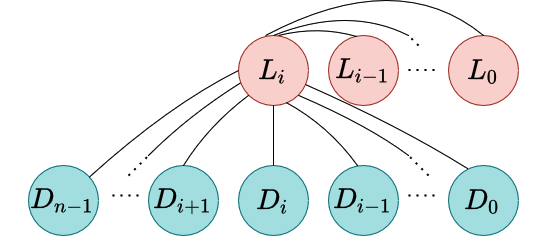
\includegraphics[width=\textwidth]{Chapter1/figures/fulldependencies.png}
	\end{subfigure}%
	\quad
\begin{subfigure}{0.31\textwidth}
	\includegraphics[width=\textwidth]{Chapter1/figures/Dual-Glowdependencies.png} 
\end{subfigure}%
\quad 
\begin{subfigure}{0.31\textwidth}
	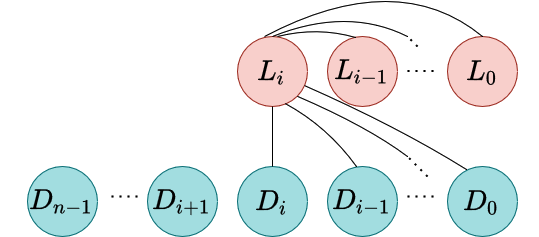
\includegraphics[width=\textwidth]{Chapter1/figures/oursdependencies.png}
	\end{subfigure}
\caption{From left to right: ideal dependencies in the $i^{th}$ autoregressive component. Dual-Glow modeling assumption \cite{Dual-Glow}; information is exchanged only between latent spaces having the same dimension. Our modeling assumption; we retain the dependencies between $L_i$ and the latent spaces of lower dimension.}	\label{ch1:fig:dependencies}
\end{figure}

The conditional distribution $P(\tilde{L}_n| \tilde{D}_n)$ is factorized using the chain rule of probability into $n$ autoregressive component distributions as shown in \eqref{ch1:conditional-distribution-autoregressive-factorization}:
\begin{equation}\label{ch1:conditional-distribution-autoregressive-factorization}
    P(\tilde{L}_n| \tilde{D}_n) = \prod_{i=0}^{n-1}P(L_i|\tilde{L}_{i},D_{n-1},...,D_0)
\end{equation}
with the notational convention that $\tilde{L}_{0}=\emptyset$ and $\tilde L_{i} = [L_{i-1}, \ldots, L_0]$ for every $i$. The dependencies of the $i^{th}$ component distribution are shown graphically in the left diagram of Figure \ref{ch1:fig:dependencies}. Modeling those $n$ autoregressive distributions can be unnecessarily computationally expensive. For this reason, we assume that 
\begin{equation}\label{ch1:eq:factorization}
    P(\tilde{L}_n| \tilde{D}_n)= \prod_{i=0}^{n-1}P(L_i|\tilde{L}_{i},\tilde D_{i+1}),
\end{equation}
where $\tilde D_{i+1} = [D_{i}, \ldots, D_0]$. In particular, we retain the dependencies between $L_{i}$ and all $L$ and $D$ latent variables of level $i$ and below, which effectively means that we are pruning only the dependencies between  $L_{i}$ and $D_{i+1},...,D_{n-1}$. We advocate that this is a valid assumption, because the encoded information in the split variables of the multi-scale flow typically ranges from local noise patterns and image details to higher-level information as we move from the early split variables to the final split variables.  The hierarchical representation in multi-scale normalizing flows is attributed to the interplay of depth of computation and the information bottleneck. We refer the reader to Appendix \ref{ch1:Hierarchical-Representation-in-Multi-Scale-Normalizing-Flows} for a more detailed discussion. \\ \color{black}
We remark that our modeling assumption is weaker than the one implicitly used in \cite{Dual-Glow} described in \eqref{ch1:eq:Dual-Glowdep} (see Figure \ref{ch1:fig:dependencies}). Precisely we allow information to be exchanged between latent spaces of different dimension. As we will demonstrate in the experiments our choice allows for more expressive architectures able to capture correlations between different scales.
We represent schematically in Figure \ref{ch1:fig:dependencies} the difference between the theoretical latent space dependencies, the one assumed in \cite{Dual-Glow} and our modeling choice. 
Under this modeling assumption, our goal is to estimate the conditional distributions $P(L_i|\tilde{L}_{i},\tilde D_{i+1})$ for every $i$ and then recover 
$P(\tilde{L}_n| \tilde{D}_n)$ using \eqref{ch1:eq:factorization}.

\subsection{Modeling the autoregressive components using conditional normalizing flows}\label{ch1:Autoregressive-conditional-flow-components}
%
%We propose to estimate each autoregressive component $P(L_i|\tilde{L}_{i},\tilde D_{i+1})$ using a multi-scale conditional normalizing flow architecture.

Modeling the autoregressive components $P(L_i|\tilde{L}_{i},\tilde D_{i+1})$ in a computationally efficient way is challenging because of the dependence on the multiple latent factors of different dimension that encode different semantic content. We propose to estimate each autoregressive component $P(L_i|\tilde{L}_{i},\tilde D_{i+1})$ with a novel multiscale normalizing flow architecture that efficiently incorporates the latent conditions. \color{black}For every $i=0, \ldots, n-1$ we define a sequence of latent variables $\tilde Z_{i+1} := [Z_{i}^{i},...,Z_0^{i}]$ defined on latent spaces of decreasing dimension $\tilde{\mathcal{Z}}_{i+1} := [\mathcal{Z}_{i}^{i},...,\mathcal{Z}_0^{i}]$ and a parametrized transformation

\begin{align*}
    G^\theta_i : \tilde{\mathcal{Z}}_{i+1} \times  \tilde{\mathcal{D}}_{i+1} \times  \tilde{\mathcal{L}}_{i} \rightarrow \mathcal{L}_{i}.
    \end{align*}
    The transformations $G^\theta_i$ are constructed by assembling multi-scale transformations $(g_j^i)_{j=0}^i$ (implicitly depending on the parameter $\theta$) defined as follows:
    \begin{align*}
    &g_0^i : \mathcal{Z}_0^i \times \mathcal{D}_0 \times \mathcal{L}_0 \rightarrow \mathcal{Z}_{0}^{\prime i} \\   
     &  g_{j}^{i}:\mathcal{Z}_{j-1}^{\prime i}\times \mathcal{Z}_{j}^{i} \times \mathcal{D}_{j} \times  \mathcal{L}_{j} \rightarrow \mathcal{Z}_{j}^{\prime i}\, \quad \text{for} \quad j=1,...,i-1\\
    &g_{i}^{i}: \mathcal{Z}_{i-1}^{\prime i}\times \mathcal{Z}_{i}^i \times \mathcal{D}_{i} \rightarrow     \mathcal{L}_{i}
\end{align*}

where $\mathcal{Z}_{i-1}^{\prime i}, \ldots, \mathcal{Z}_0^{\prime i} $ are intermediate latent spaces of decreasing dimension, $g_j^i$ is invertible as a function from $\mathcal{Z}_{j-1}^{\prime i} \times \mathcal{Z}_{j}^i$ to $\mathcal{Z}_{j}^{\prime i}$ and $g_0^i$  is invertible as function from $\mathcal{Z}_0^i$ to $\mathcal{Z}_{0}^{\prime i}$.
The transformation $G^\theta_i$ is then obtained by composing the functions  $g_{j}^{i}$ in the following way. Given the conditioning variables $(\de_j)_{j=0}^i \in \tilde{\mathcal{D}}_{i+1}$ and $(\el_j)_{j=0}^{i-1} \in \tilde{\mathcal{L}}_{i}$, a latent variable $\z_0 \in \mathcal{Z}_0^i$ is transformed to $\z_0' \in \mathcal{Z}_0^{\prime i}$ by function $g^i_0(\cdot ; \de_0, \el_0)$. 
Then $\z_0'$ and $\z_1$ are concatenated and inserted to $g^i_1(\cdot;\de_1, \el_1)$ which outputs $\z_1' \in \mathcal{Z}_1^{\prime i}$. This process continues as implied up until the $i^{th}$ level whose output is $\el_i = g_i^i(\z_{i-1}', \z_i; \de_i) \in \mathcal{L}_{i}$. A schematic description of $G^\theta_i$ is presented in the right diagram of Figure \ref{ch1:fig:high_level_design_conditional}. 

Denote by $f_{j}^{i}$ (implicitly depending on the parameter $\theta$) the inverse of $g_{j}^{i}$ for fixed conditioning variables in $\mathcal{D}_j$ and $\mathcal{L}_j$
\begin{align*}
&f_0^i : \mathcal{Z}_0^{\prime i} \times \mathcal{D}_0 \times \mathcal{L}_0 \rightarrow \mathcal{Z}_0^i \\   
 &  f_{j}^{i}:  \mathcal{Z}_{j}^{\prime i} \times \mathcal{D}_{j} \times  \mathcal{L}_{j} \rightarrow \mathcal{Z}_{j-1}^{\prime i}\times  \mathcal{Z}_{j}^i\, \quad \text{for} \quad j=1,...,i-1\\
&f_{i}^{i}:    \mathcal{L}_{i} \times \mathcal{D}_{i} \rightarrow  \mathcal{Z}_{i-1}^{\prime i}\times \mathcal{Z}_{i}^i
\end{align*}
and by $F_i^\theta$ the inverse of $G_i^\theta$ as a function from $\tilde{\mathcal{Z}}_{i+1}$ to $\mathcal{L}_i$ obtained by composing the functions $f^i_j$ for $j = 0, \ldots, i$.
We model each $f_{j}^{i}$ by adopting the conditional flow design of \cite{SRFLOW}. More specifically, we initially use the same squeeze layer, which is followed by two transition steps and $K$ conditional flow steps. Each transition step consists of an actnorm layer followed by $1\times1$ invertible convolution layer. Each conditional flow step consists of an actnorm layer followed by $1\times1$ invertible convolution, which is followed by an affine injector and an affine coupling layer. We use from 8 to 16 conditional flow steps depending on the difficulty of the image translation task.

\smallskip

\textbf{A discussion on sharing weights strategies.} It is worth noting that the multi-scale transformations, denoted as \(g_j^i\), for all transformations \(G_i^{\theta}\) where \(i \geq j+1\), share the same architecture and function – integrating information from conditions \(D_j\) and \(L_j\). This hints at the potential of utilizing a singular subflow, \(g_j^{j+1}\), for every \(G_i^{\theta}\) with \(i \geq j+1\). Such a strategy could decrease the computational burden and introduce an inductive bias. Yet, it is crucial to recognize that this approach assumes the only distinctive subflow in each \(G_i^{\theta}\) flow is \(g_i^i\). All the deeper subflows, represented by \(g_k^i\) where \(k<i\), are shared between \(G_i^{\theta}\) and other \(G_j^{\theta}\) flows. This results in a modeling constraint, narrowing the space of functions the architecture can represent. Our preliminary tests confirmed this limitation; the performance using this approach significantly lags behind the more generalized model presented in this chapter.

\begin{figure}[t]
    \centering
    \begin{subfigure}{0.45\textwidth}
        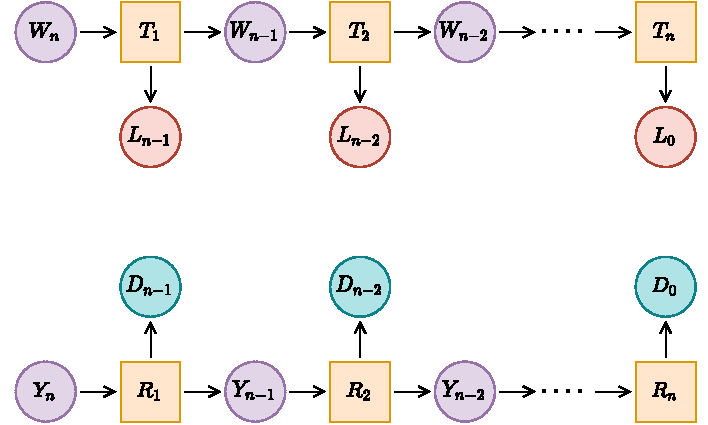
\includegraphics[width=\textwidth]{Chapter1/figures/dual_glow.pdf}
    \end{subfigure}%
    \qquad 
    \begin{subfigure}{0.47\textwidth}
            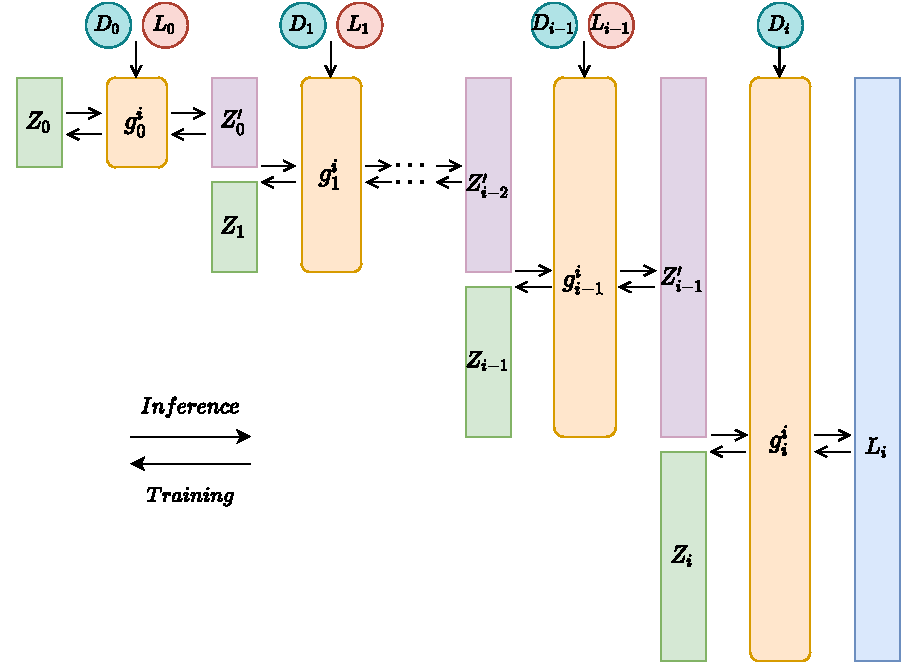
\includegraphics[width=\textwidth]{Chapter1/figures/high_level_design_conditional_modified.pdf}
    \end{subfigure}
    \caption{Left: unconditional normalizing flow architecture used to encode conditioning and conditioned images, denoted by $Y_n = Y$ and $W_n = W$ respectively, into a sequence of hierarchical latent variables. Right: design of the conditional transformation $G_{i}^\theta$ that models the $i^{th}$ autoregressive component. The index of the flow $i$ is omitted in both the transformed latent variable $Z_j$ and the intermediate latent variables $Z_j^{\prime}$ for simplicity.}
           \label{ch1:fig:high_level_design_conditional}
\end{figure}

\subsection{Maximum log-likelihood estimation and training}
Here we use the constructed transformations $G_i^\theta : \tilde{\mathcal{Z}}_{i+1} \times  \tilde{\mathcal{D}}_{i+1} \times  \tilde{\mathcal{L}}_{i} \rightarrow \mathcal{L}_{i}$ to parametrize each autoregressive component $P(L_i|\tilde{L}_{i},\tilde D_{i+1})$ and, together with the unconditional normalizing flows $R^{\theta} := R^\theta_n \circ \ldots \circ R^\theta_1$ and $T^{\theta}:= T^\theta_n \circ \ldots \circ T^\theta_1$, use them to estimate $P(W|Y)$. To model $ P(\tilde{L}_n| \tilde{D}_n)$ through its autoregressive componenents as in \eqref{ch1:conditional-distribution-autoregressive-factorization}, we define 
the operator $G^\theta : \tilde{\mathcal{Z}}_{1} \times \ldots \times \tilde{\mathcal{Z}}_{n} \times  \tilde{\mathcal{D}}_{n}  \rightarrow \tilde{\mathcal{L}_{n}}$ as the concatenation of the operators $G^\theta_i$ defined in the previous section, i.e. 
\begin{align}\label{ch1:eq:G}
    G^\theta = [G^\theta_0, \ldots, G^\theta_{n-1}].
\end{align}
where $G^\theta_i$ is computed inductively using $G^\theta_j$ for $j<i$ as in the autoregressive factorization \eqref{ch1:conditional-distribution-autoregressive-factorization}.
Then we consider the map $H^\theta :  \tilde{\mathcal{Z}}_{1} \times \ldots \times \tilde{\mathcal{Z}}_{n} \times \mathcal{Y}\rightarrow \mathcal{W}$ defined as  $H^\theta(\tilde \z_1, \ldots, \tilde \z_n, \y):= (T^\theta)^{-1}( G^\theta(\tilde \z_1, \ldots, \tilde \z_n ; R^\theta(\y)))$ and we denote by $p^\theta_{W|Y}$ the distribution of the pushforward measure
\begin{align}
    H^\theta_\#(\cdot, \y) P([\tilde Z_{1}, \ldots, \tilde Z_{n}]).
\end{align}
We minimize the negative log-likelihood of $p^\theta_{W|Y}$ to obtain an estimate of $P(W|Y)$.
With this aim, for every latent variable $Z_j^i$ in $\tilde Z_j$ we choose as prior a multivariate normal distribution, whose density we denote by $\mathcal{N}(\cdot; \textbf{0}, \textbf{I})$.
In the next theorem we provide an explicit formula for the logarithm of $p^\theta_{W|Y}$ expressed in terms of $R^\theta_i$, $T^\theta_i$ and $f^i_j$.

\begin{proposition}
    The logarithm of $p^\theta_{W|Y}$ can be computed as
    \begin{align}
    \log p^\theta_{W|Y}(\boldsymbol{w} | \y)   & = \sum_{i=1}^{n}\log{\Bigg|{\rm det}\frac{\partial T_i^{\theta}(\boldsymbol{w}_{n-i+1})}{\partial \boldsymbol{w}_{n-i+1}}\Bigg|} \nonumber \\ 
    & + \sum_{i=1}^{n-1} \sum^{i-1}_{j=0} \left[\log \mathcal{N}(\z_j^i;\textbf{0},\textbf{I})+\log \Bigg|{\rm det}\left(\frac{\partial f^i_{j}(\z_j^{\prime i};\el_j,\de_{j})}{\partial \z_j^{\prime i}}\right)\Bigg|\right] \nonumber\\
    & + \sum_{i=0}^{n-1}  \left[\log \mathcal{N}(\z_i^i;\textbf{0},\textbf{I})+\log \Bigg|{\rm det}\left(\frac{\partial f^i_{i}(\el_{i};\de_{i})}{\partial \el_{i}}\right)\Bigg|\right]\label{ch1:eq:obj}
    \end{align} 
    
    where the normal distributions are computed in the latent variables $\z_j^i = f_j^i(\z_j^{\prime i}, \boldsymbol{d}_j,\boldsymbol{l}_j)$ and $\z_i^i = f_i^i( \boldsymbol{d}_i,\boldsymbol{l}_i)$. Moreover, each intermediate latent variable $\z_j^{\prime i}$ is defined recursively by the application of the previous $f_j^i$ (see Figure \ref{ch1:fig:high_level_design_conditional}) and ${\de}_{i} \in \mathcal{D}_{i}$ implicitly depend on $\y \in Y$ through the normalizing flow $R^\theta$. 
    
\end{proposition}

\begin{proof}
    First we express the logarithm of $p^\theta_{W|Y}$ in terms of $p^\theta_{\tilde{L}_n|\tilde{D}_n}$, where  $p^\theta_{\tilde{L}_n|\tilde{D}_n}$ is the distribution induced by the map $G^\theta$ defined in \eqref{ch1:eq:G}. We obtain
    \begin{equation}\label{ch1:eq:equationone}
    \begin{aligned}
         \log p^\theta_{W|Y}(\boldsymbol{w} | \y)=& \log \Big|\text{det}\Bigg(\frac{\partial T^\theta(\boldsymbol{w})}{\partial \boldsymbol{w}}\Bigg)\Big| + \log{p^\theta_{\tilde{L}_n|\tilde{D}_n}(\tilde{\el}_n|\widetilde{\de}_n)} \\ 
        =& \sum_{i=1}^{n}\log{\Bigg|\text{det}\frac{\partial T_i^{\theta}(\boldsymbol{w}_{n-i+1})}{\partial \boldsymbol{w}_{n-i+1}}\Bigg|}+ \log{\prod_{i=0}^{n-1}p^\theta_{L_i|\tilde{L}_{i},\tilde D_{i+1}}(\el_i|\tilde{\el}_{i},\widetilde \de_{i+1})} \\
        =& \sum_{i=1}^{n}\log{\Bigg|\text{det}\frac{\partial T_i^{\theta}(\boldsymbol{w}_{n-i+1})}{\partial \boldsymbol{w}_{n-i+1}}\Bigg|}+ \sum_{i=0}^{n-1}\log{p_{L_i|\tilde{L}_{i},\tilde D_{i+1}}^\theta(\el_i|\tilde{\el}_{i},\widetilde \de_{i+1})}.
    \end{aligned}
    \end{equation}
    
    The justification for the first line can be found in  \cite[Section 3]{Dual-Glow}. In the second line we use the chain rule for distribution and we factorize the conditional distribution using the dependency assumptions of our model. Now observe that
    
    \begin{equation}\label{ch1:eq:equationtwo}
    \begin{aligned}
        \sum_{i=0}^{n-1}\log{p_{L_i|\tilde{L}_{i},\tilde D_{i+1}}^\theta(\el_i|\tilde{\el}_{i},\widetilde \de_{i+1})}
         =& \sum_{i=0}^{n-1}\log{p_{\tilde{Z}_{i+1}}(F_i^{\theta}(\el_i;\tilde{\el}_{i},\widetilde \de_{i+1}))}\\
         &  +\log{\Bigg|\text{det}\frac{\partial F_i^{\theta}(\el_i;\tilde{\el}_{i},\widetilde \de_{i+1})}{\partial \el_i}\Bigg|} \\
        =& \sum_{i=1}^{n-1} \sum^{i-1}_{j=0} \Bigg[\log \mathcal{N}(\z_j^i;\textbf{0},\textbf{I})\\
        &  +\log \Bigg|\text{det}\left(\frac{\partial f^i_{j}(\z_j^{\prime i};\el_j,\de_{j})}{\partial \z_j^{\prime i}}\right)\Bigg|\Bigg] \\
    & + \sum_{i=0}^{n-1}  \left[\log \mathcal{N}(\z_i^i;\textbf{0},\textbf{I})+\log \Bigg|\text{det}\left(\frac{\partial f^i_{i}(\el_{i};\de_{i})}{\partial \el_{i}}\right)\Bigg|\right],
    \end{aligned}
    \end{equation}
    where the normal distributions are computed in the latent variables $\z_j^i = f_j^i(\z_j^{\prime i}, \boldsymbol{d}_j,\boldsymbol{l}_j)$ and $\z_i^i = f_i^i( \boldsymbol{d}_i,\boldsymbol{l}_i)$.
    The first line of \eqref{ch1:eq:equationtwo} is obtained by using the change-of-variables formula. In the second line we use the chain rule for the composition of functions using the definition of $F_{i}^{\theta}$ in \ref{ch1:Autoregressive-conditional-flow-components} and the assumption that the latent variables $Z_i^i,Z_{i-1}^i, ..., Z_0^i$ which comprise $\tilde{Z}_{i+1}$ are i.i.d. with distribution $\mathcal{N}(\textbf{0},\textbf{I})$. The sum is then broken into two sums, because the $f_i^i$ functions are conditioned only on $\de_i$ by definition. Therefore, combining \eqref{ch1:eq:equationone} and \eqref{ch1:eq:equationtwo} we obtain
    
    \begin{align}
    \log p^\theta_{W|Y}(\boldsymbol{w} | \y)   & = \sum_{i=1}^{n}\log{\Bigg|\text{det}\frac{\partial T_i^{\theta}(\boldsymbol{w}_{n-i+1})}{\partial \boldsymbol{w}_{n-i+1}}\Bigg|} \nonumber \\ 
    & + \sum_{i=1}^{n-1} \sum^{i-1}_{j=0} \left[\log \mathcal{N}(\z_j^i;\textbf{0},\textbf{I})+\log \Bigg|\text{det}\left(\frac{\partial f^i_{j}(\z_j^{\prime i};\el_j,\de_{j})}{\partial \z_j^{\prime i}}\right)\Bigg|\right] \nonumber\\
    & + \sum_{i=0}^{n-1}  \left[\log \mathcal{N}(\z_i^i;\textbf{0},\textbf{I})+\log \Bigg|\text{det}\left(\frac{\partial f^i_{i}(\el_{i};\de_{i})}{\partial \el_{i}}\right)\Bigg|\right] \nonumber
    \end{align} 
    as we wanted to prove.
    
\end{proof}

We train our CAFLOW model by minimizing the following training objective \begin{align*}
        \log p^\theta_{W|Y}(\boldsymbol{w} | \y) + \lambda \log p^\theta_{Y}(\y),
        \end{align*}
        where $p^\theta_{Y}(\y)$ is estimated using the unconditional normalizing flow $R^\theta$ as in Subsection \ref{ch1:subsec:normalizing}.
        The parameter $\lambda$ interpolates between the conditional distribution $P(W|Y)$ (when $\lambda = 0$) and the joint distribution $P(Y,W)$ (when $\lambda = 1$).
        Indeed, if $\lambda = 1$ the objective can be written as
        \begin{align}
        \log p^\theta_{W|Y}(\boldsymbol{w} | \y) +  \log p^\theta_{Y}(\y) = \log (p^\theta_{W|Y}(\boldsymbol{w} | \y)p^\theta_{Y}(\y)) = \log\left(p^\theta_{Y,W}(\y,\boldsymbol{w})\right)
        \end{align}
        where $p^\theta_{Y,W}$ is the density of the joint distribution $P(Y,W)$.
        Note that $\lambda$ can be interpreted as a regularization parameter. This intuition is justified noticing that if $\lambda = 1 - \varepsilon$ for $\varepsilon \in [0,1]$ we can write
        \begin{align}
           \log p^\theta_{W|Y}(\boldsymbol{w} | \y) +  (1-\varepsilon) \log p^\theta_{Y}(\y) =  \log(p^\theta_{Y,W}(\y,\boldsymbol{w})) + \log\left(\frac{1}{(p^\theta_Y(\y))^\varepsilon}\right)  
        \end{align}
        where the term $\log(\frac{1}{(p^\theta_Y(\y))^\varepsilon})$ 
        is close to infinity in the regions where $p^\theta_Y(\y)$ is small, that are the unlikely images in the distribution. By choosing $\varepsilon < 1$ instead of $\varepsilon \sim 1$ the term $\log(\frac{1}{(p^\theta_Y(\y))^\varepsilon})$ becomes smaller in such regions by improving the stability of the training process. 
    

\subsection{Inference}

The standard way to perform inference using a trained CAFLOW model is the following: 
\begin{enumerate}
        \item Calculate the conditional encodings $(\de_{n-1},...,\de_0) \in \tilde{\mathcal{D}}_n$ by passing the conditioning image through the unconditional multi-scale flow $R^\theta$.
        \item Sample latent variables $\z_i^j$ from $\mathcal{N}(\textbf{0},\tau^2 \textbf{I})$, where $0<\tau \leq 1$ denotes the sampling temperature.
        \item Calculate the output image latent variables $\el_0,...,\el_{n-1} \in \tilde{\mathcal{L}}_n$ by applying the transformations $G^\theta_i$ sequentially from $G^\theta_0$ to $G^\theta_{n-1}$.
        \item Finally, convert the output image latents $\el_0,...,\el_{n-1}$ to the output image by passing them through the unconditional reverse normalizing flow $(T^\theta)^{-1}$.
\end{enumerate}

\textbf{Sampling temperature $\tau$ and its importance}. During training, we set \( \tau = 1 \). However, for sampling, we adopt a reduced temperature \( \tau <1 \).

Despite sampling from a slightly different distribution than the one that we learnt, this choice enhances the quality of the output image reducing the occurrence of severe artifacts.

The challenge with many normalizing flow architectures, including ours, lies in their structure: composing numerous analytically bi-Lipschitz functions increases the Lipschitz coefficient of the inverse flow, as detailed by \cite{behrmann2021understanding} and \cite{verine2023expressivity}. The amplification of the Lipschitz constant compromises the numerical stability of the inverse flow which is used for sampling.
Empirically, a lower sampling temperature ensures better numerical stability, which implies that the Lipschitz constant of the inverse flow constrained in the higher density regions is significantly smaller. 

The choice of $\tau$ for sampling is crucial in this regard. For $\tau < 1$ we gain a better numerical stability while we could lose accuracy as a consequence of sampling from a different distribution. This trade-off can be quantified (for instance) in terms of the $2$-Wasserstein distance between the distributions generated by the normalizing flow $G$ for different levels of $\tau$ as follows: 
\begin{align*}
    W_2(G_\# \mathcal{N}(0,\textbf{I}), G_\# \mathcal{N}(0,\tau \textbf{I})) & \leq {\rm Lip}(G) W_2(\mathcal{N}(0,\textbf{I}), \mathcal{N}(0,\tau \textbf{I})) \\
    & \leq {\rm Lip}(G) \sqrt{d(1 + \tau - 2\sqrt{\tau})}
 \end{align*}
where ${\rm Lip}(G)$ is the Lipschitz constant of $G$, $G_\# \mu$ is the push-forward of the probability measure $\mu$ by $G$ and $d$ is the dimension of the normal distributions. In particular, since the sampling error is amplified by the Lipschitz constant of the normalizing flow, the interplay between accuracy and numerical stability that is regulated by the choice $\tau$ is complex and heavily depends on the data distribution and on the learnt normalizing flow.  

Finally, we mention that alternative methods based either on the regularization of the training objective \cite{onken2021ot} or on a priori controls of the Lipschitz constant of the flow (and its inverse) \cite{verine2023expressivity} might achieve similar outcomes to adjusting the sampling temperature. Such approaches, however, come with additional computational challenges and their analysis fall beyond the scope of this study.

\smallskip

\textbf{Optimized sample selection using conditional likelihood estimation}. \color{black}Our framechapter can act both as conditional generator and as a conditional likelihood estimator. Figure \ref{ch1:fig:decreasingloglikelihood} shows ten super-resolved versions of the low resolution image in decreasing order of conditional log-likelihood. We leverage the conditional likelihood estimation to automatically select the best generated samples and disregard bad samples. 

\begin{figure}[h!]
    \centering
    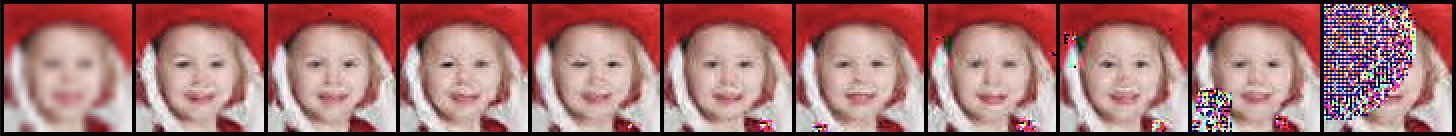
\includegraphics[width=\textwidth]{Chapter1/paper_graphs/10samples_decreasing_conditional_loglikelihood.png}
    \caption{10 super-resolved versions of the LR image in decreasing conditional log-likelihood order.}
    \label{ch1:fig:decreasingloglikelihood}
\end{figure}

We have observed that CAFLOW typically assigns to the ground-truth image higher conditional log-likelihood than any generated sample. Such observation suggests that CAFLOW is a powerful conditional likelihood estimator, and that better samples can be obtained by the use of an optimisation algorithm, which searches for samples with high conditional likelihood. However, we used a simpler inference method in this chapter: keep the best $N$ out of $M$ generated samples based on the conditional log-likelihood. We empirically found that $M$ should be larger for higher sampling temperatures.

\section{Experiments}\label{ch1:sec:numerics}
In this section we evaluate CAFLOW on three image-to-image translation tasks: image super-resolution, image colorization and image inpainting. Moreover, as ablation for the autoregressive structure in a image super-resolution task, we compare CAFLOW to a model that is conditioned in the normalizing flow latent space, assuming that information is exchanged only between latent spaces having the same dimension, c.f. Section \ref{ch1:subsec:modass} and Figure \ref{ch1:fig:dependencies}. 

We refer the reader to section \ref{ch1:sec:details-of-experiments} in the Appendix for more details about the reported experiments and to section \ref{ch1:sec:extended-visual-results} for extended visual results.

\subsection{Image Super-resolution}
\subsubsection{Ablation of the autoregressive structure}
The idea of conditioning in the normalizing flow latent space was first introduced in \cite{Dual-Glow} to design a conditional likelihood estimator named Dual-Glow. 
The main advantage of CAFLOW compared to Dual-Glow is the autoregressive structure in the latent space that allows to accommodate information exchange at different scales. We confirmed it experimentally by pruning the autoregressive connections and modeling the Dual-Glow component distribution $p(L_i|D_i)$ with a conditional normalizing flow. We named this model Dual-Glow+ as it has the same modeling structure as Dual-Glow with the extra advantage of modeling the component distribution $p(L_i|D_i)$ with a conditional normalizing flow instead of a multidimensional Gaussian distribution as in  \cite{Dual-Glow}. Moreover, we increased the depth of the conditional flow that models $p(L_i|D_i)$, so that Dual-Glow+ and CAFLOW have approximately the same number of parameters. This is important to ensure that improved performance of CAFLOW is the result of the autoregressive modeling structure.

\begin{figure}[h!]
    \begin{center}
    \setlength{\tabcolsep}{0pt}
    \begin{tabular}{cccccc}
        \scriptsize LR   &  \scriptsize Bicubic & \scriptsize Dual-Glow+    &  \scriptsize  \textbf{CAFLOW}     & \scriptsize True \\
          & (x4) & (x4)    & (x4) & 1024x1024 \\
    
    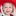
\includegraphics[width=0.18\linewidth]{Chapter1/paper_graphs/super_resolution/LR.jpg} &
    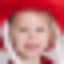
\includegraphics[width=0.18\linewidth]{Chapter1/paper_graphs/super_resolution/BICUBIC.jpg} &
    \includegraphics[width=0.18\linewidth]{Chapter1/paper_graphs/super_resolution/Dual-Glow.png} &
    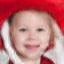
\includegraphics[width=0.18\linewidth]{Chapter1/paper_graphs/super_resolution/CAFLOW.png} &
    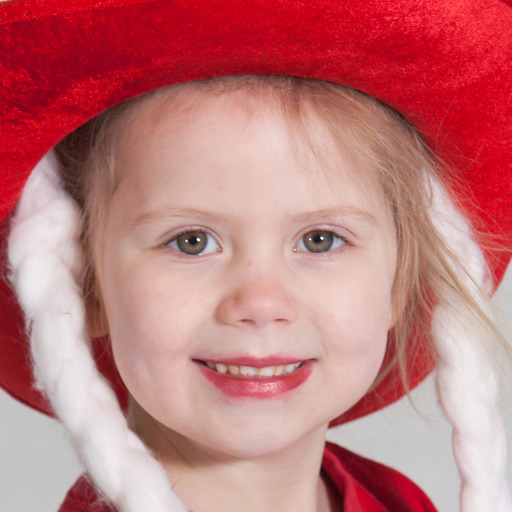
\includegraphics[width=0.18\linewidth]{Chapter1/paper_graphs/super_resolution/TRUE.jpg} \\
    
    \end{tabular}
    \caption{Qualitative comparison of Dual-Glow+ and CAFLOW.}
    \label{ch1:fig:ablation}
    \end{center}
\end{figure}

In Figure \ref{ch1:fig:ablation} we show the qualitative comparison of Dual-Glow+ and CAFLOW on a x4 super-resolution task.  It is apparent that CAFLOW outperforms Dual-Glow+, confirming the significance of allowing exchange of information between different scales. We refer to the next section for more details about the image super-resolution experiment and a quantitative comparison between Dual-Glow+ and CAFLOW, c.f. Table \ref{ch1:comparisonBRGM}.

\subsubsection{Experiment}
We evaluate the ability of CAFLOW and Dual-Glow+ to perform image super-resolution on the FFHQ dataset \cite{karras2019style} (Creative Commons BY-NC-SA 4.0). We resized the original images to $16\times16$ and $64\times 64$ patches and trained the model for x4 super-resolution. The quantitative evaluation is performed using the LPIPS and RMSE scores on 100 unseen images. For inference, we used $\tau=0.5$ and kept the sample with the highest conditional log-likelihood out of ten generated samples. A comparison with state-of-the-art methods is shown in Table \ref{ch1:comparisonBRGM}. We present visual results in Figure \ref{ch1:SR-visuals-paper} and refer the reader to the supplementary material for more examples.

{\footnotesize
\begin{table}[h!]
\centering
\caption{Quantitative evaluation of (x4) super-resolution on FFHQ $16^2$. We report LPIPS/RMSE scores for each method. Lower scores are better.}\label{ch1:comparisonBRGM}
\label{ch1:eval-super-resolution}
\setlength{\tabcolsep}{3pt}


\begin{tabular}{l|cccccc}\label{ch1:tab:one}
 Dataset &    \textbf{CAFLOW} & \textbf{Dual-Glow+} &   BRGM \cite{BRGM}     &   ESRGAN \cite{ESRGAN}    &   SRFBN \cite{li2019feedback}  &  BICUBIC \\

%  & \lpi & \rms  & \lpi & \rms & \lpi & \rms & \lpi & \rms\\
\midrule
   FFHQ $16^2$ &  \textbf{0.08}/\textbf{17.56}  &  \textbf{0.14}/\textbf{18.56} & 0.24/25.66  &  0.35/29.32 &  0.33/22.07 & 0.34/20.10 \\

\end{tabular}
%\vspace{0.1in}
\end{table}
}

\begin{figure}[h!]
    \begin{center}
    \setlength{\tabcolsep}{1pt} % Optional: Adjust the space between images
    \begin{tabular}{cccccccc}
        \scriptsize LR & \scriptsize Bicubic & \scriptsize ESRGAN & \scriptsize SRFBN & \scriptsize BRGM & \scriptsize Dual-Glow+ & \scriptsize \textbf{CAFLOW} & \scriptsize True \\
        & (x4) & (x4) & (x4) & (x4) & (x4) & (x4) & 1024x1024 \\
        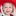
\includegraphics[width=0.12\linewidth]{Chapter1/paper_graphs/super_resolution/LR.jpg} &
        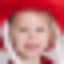
\includegraphics[width=0.12\linewidth]{Chapter1/paper_graphs/super_resolution/BICUBIC.jpg} &
        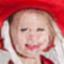
\includegraphics[width=0.12\linewidth]{Chapter1/paper_graphs/super_resolution/ESRGAN.jpg} &
        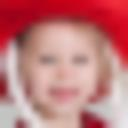
\includegraphics[width=0.12\linewidth]{Chapter1/paper_graphs/super_resolution/SRFBN.jpg} &
        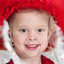
\includegraphics[width=0.12\linewidth]{Chapter1/paper_graphs/super_resolution/BRGM.jpg} &
        \includegraphics[width=0.12\linewidth]{Chapter1/paper_graphs/super_resolution/Dual-Glow.png} &
        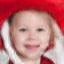
\includegraphics[width=0.12\linewidth]{Chapter1/paper_graphs/super_resolution/CAFLOW.png} &
        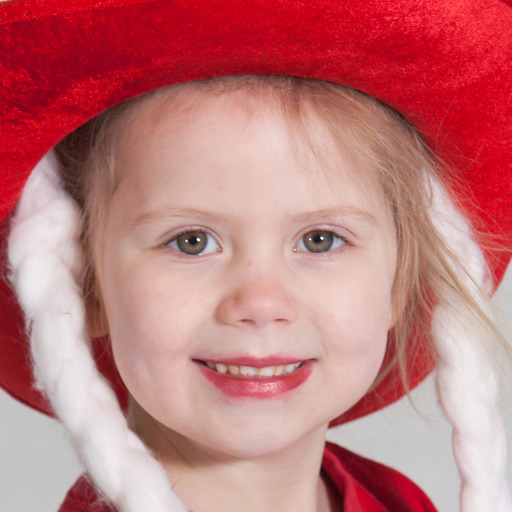
\includegraphics[width=0.12\linewidth]{Chapter1/paper_graphs/super_resolution/TRUE.jpg} \\
    \end{tabular}
    \end{center}
    \caption{Qualitative evaluation on FFHQ 4x super-resolution of 16x16 resolution images.}\label{ch1:SR-visuals-paper}
    \end{figure}
    
    Table \ref{ch1:comparisonBRGM} shows that CAFLOW outperforms Dual-Glow+ based on both metrics, which confirms the theoretical advantage of the autoregressive modeling structure. Moreover CAFLOW outperforms all the other super-resolution methods based on both metrics. It is slightly inferior to BRGM \cite{BRGM} in terms of perceptual quality but it is significantly better in terms of fidelity which is reflected in the quantitative evaluation.


\subsection{Image Colorization}
    To our knowledge, diverse image colorization has been addressed by conditional flows \cite{ardizzone2019guided}, conditional GANs \cite{colorGAN} and recently score-based models \cite{scorebased}. 
    We trained the model on $10\%$ of the LSUN bedroom $64\times 64$ training dataset \cite{yu2015lsun},  a popular dataset for image colorization. For inference, we used $\tau=0.85$ and kept the best out of ten generated samples for each test image using the conditional log-likelihood. We report the performance of the model in Table \ref{ch1:colorisation-comparison}. We use the FID score to compare our method against the cINN and ColorGAN, which have been trained on the full dataset. We show visual results for all methods in Figure \ref{ch1:fig:colorisation-paper-visuals-results}. 
    We did not include \cite{scorebased} in the comparison because it was trained on higher resolution images.

\begin{figure}[h!]
        \begin{center}
        \setlength{\tabcolsep}{3pt}
        %\renewcommand{\arraystretch}{1.5}% Spread rows out...
        \begin{tabular}{ccc}
        CAFLOW & CINN \cite{ardizzone2019guided} & ColorGAN \cite{colorGAN}  \\
        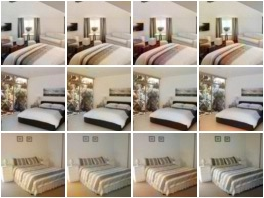
\includegraphics[height=2.9cm]{Chapter1/paper_graphs/colourisation/CAFLOW_borders.png}&
        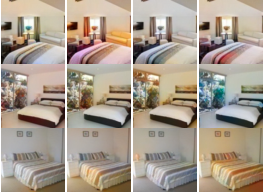
\includegraphics[height=2.9cm]{Chapter1/paper_graphs/colourisation/CINN.png}&
        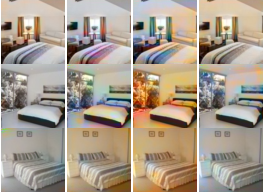
\includegraphics[height=2.9cm]{Chapter1/paper_graphs/colourisation/colorGAN.png}\\
        \end{tabular}
        \caption{Qualitative evaluation: Four colorizations proposed by CAFLOW, CINN and ColorGAN for three test images. ColorGAN generates unrealistically diverse colorizations with significant color artifacts (for example a yellow region on a white wall). CINN generates more realistic, less diverse colorizations with fewer pronounced color artifacts compared to ColorGAN, which is reflected in the improved FID score. Finally, CAFLOW generates even more realistic and less diverse colorizations than CINN with even rarer color artifacts, which is more representative of the data distribution according to the FID score.}
        \label{ch1:fig:colorisation-paper-visuals-results}
        \end{center}
\end{figure}

\begin{table}[h!]
    \centering
    
    \caption{Quantitative evaluation of colorization on LSUN BEDROOM $64\times 64$ dataset. We report FID score for each method. Lower scores are better. }
    \label{ch1:colorisation-comparison}
    \setlength{\tabcolsep}{3pt}
    
    \begin{tabular}{l|ccccc}
     Metric &    \textbf{CAFLOW} &   CINN \cite{ardizzone2019guided}     &   ColorGAN \cite{colorGAN}  \\
    
    %  & \lpi & \rms  & \lpi & \rms & \lpi & \rms & \lpi & \rms\\
    \midrule
      FID &  \textbf{18.15} & 26.48 &  28.31 \\
    
    \end{tabular}
    %\vspace{0.1in}
\end{table}

Our model outperforms both methods on image colorization based on the FID metric. We calculated the FID score by generating one conditional sample for each test image, so that our evaluation is identical with the evaluation of the other methods. Moreover, we calculated the FID score by generating 5 samples for each test image, which yielded an improved FID score ($\textbf{16.73}$). We suggest that this protocol be adopted by methods which address diverse image colorization in the future. 

\subsection{Image Inpainting}

We evaluated the performance of CAFLOW on image inpainting by removing central masks covering $25\%$ of the centrally cropped human face of the CelebA dataset \cite{liu2015deep}. We compare the performance of the model with the conditional flow \cite{cGLOW} on the same task using the PSNR metric, see Table \ref{ch1:quantitative-evaluation-inpainting}. We show inpainting examples in Figure \ref{ch1:qualitative-performance-inpainting}.

\begin{figure}[h!]
    \centering
    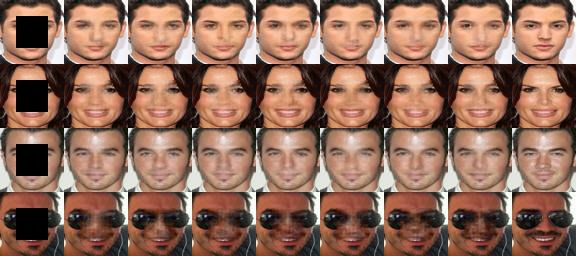
\includegraphics[width=.8\textwidth]{Chapter1/paper_graphs/inpainting/even_smaller_merged.jpg}
    \caption{Different inpaintings proposed by CAFLOW with $\tau=0.5$. Ground truth on the right.}
    \label{ch1:qualitative-performance-inpainting}
\end{figure}

Our model outperforms \cite{cGLOW} based on the PSNR metric and on qualititative performance. CAFLOW generates realistic images by blending smoothly the conditioning with the synthesized part of the image in contrast to \cite{cGLOW} which generates overly smooth synthesized parts which do not blend well with the surrounding image. Both methods fail in faces which wear sunglasses or face sidewise. We believe that this is attributed to the small number of such training examples.

\begin{table}[h!]
    \centering
    \caption{Quantitative evaluation of inpainting on the CelebA dataset. We report PSNR and LPIPS scores for each method.}\label{ch1:quantitative-evaluation-inpainting}
    \setlength{\tabcolsep}{3pt}
    \begin{tabular}{l|cccc}
     Method  &  PSNR$\uparrow$  &   LPIPS$\downarrow$    \\
    
    \midrule
      \textbf{CAFLOW} &  \textbf{26.08} & 0.06  \\
      \cite{cGLOW} & 24.88 & -
        
    \end{tabular}
    %\vspace{0.1in}
    \end{table}

\section{Conclusions}\label{ch1:sec:conclusions}

We have introduced a conditional autoregressive flow, coined CAFLOW, which combines autoregressive modeling with conditional normalizing flows for image-to-image translation. CAFLOW is an efficient conditional image generator and conditional likelihood estimator able to cross-correlate information at different scales, improving on the expressivity of former conditional flow architectures. 
We demonstrate its efficiency as conditional generator on standard image-to-image translation tasks such as image super-resolution, image colorization and image inpainting. We find that, in the above-mentioned tasks, CAFLOW achieves better performance than standard conditional flows and conditional GANs. In particular, we observe that the autoregressive modeling that allows information exchange at different scales, improves on Dual-Glow performances \cite{Dual-Glow}, where correlation is allowed only between latent spaces of the same dimension.

The main modeling limitation of the framework is attributed to limited expressivity of normalizing flows. Each transformation of a normalizing flow has to be invertible with a tractable calculation of the determinant of the Jacobian. This limits the representational power of normalizing flows. However, Wu et al. \cite{wu2020stochastic} claim to overcome expressivity limitations of normalizing flows by combining deterministic invertible functions with stochastic sampling blocks. Therefore, incorporating their proposed stochastic blocks in our conditional autoregressive flows could potentially lead to significant performance improvement. 

